\chapter{\hlc[cyan]{EVDT Framework}} \label{ch:evdt}

\section{\hlc[yellow]{Chapter Purpose \& Structure}}

The aim of this chapter is to detail a framework for developing a \acf{dss} for a sustainable development application. This framework, called the \acf{evdt} Framework, builds upon the lessons and priorities identified in Chapter \ref{ch:theory}. Compared to most frameworks for applying \acf{eo} data for sustainable development, the \ac{evdt} Framework aims to be applicable to a wider range of spatial and temporal scales (particularly on the smaller and shorter end of things); to involve a wider range of stakeholders throughout the development process; and to be attentive to both environmental and human wellness, rather than just one or the other.

The chapter starts in Section \ref{sec:intended} by walking through the proposed \ac{evdt} Framework step by step. Section \ref{sec:intended} then presents the intended uses of the framework in more detail. This is followed by Section \ref{sec:novelty} which compares the proposed frameworks to other approaches and discusses the novelty of the proposed framework. [** discuss how the remaining sections of the chapter]]. Chapters \ref{ch:mangroves} and \ref{ch:vida} will then present applied case studies of the \ac{evdt} Framework for those interested in concrete demonstrations. [** maybe mention concluding chapter(s) as well]]

This chapter aims to advance Research Question 1: 

\blockquote{\textit{What aspects of systems architecture (and systems engineering in general) are relevant and useful for approaching issues of sustainability in complex \acf{sets}? In particular, how can they be adapted using techniques from collaborative planning theory and other critical approaches to enable avoid the technocratic excesses of the past?}}

It accomplishes this by supplying Research Deliverable 1b: 

\blockquote{\textit{A proposed framework for applying systems engineering for sustainable development in an anticolonialist manner.}} 

That proposed framework is called the \ac{evdt} Framework.




\section{\hlc[yellow]{The Framework}} \label{sec:framework}

The \ac{evdt} Framework is process for developing a \ac{dss} for a sustainable development application. This processed is characterized by five basic elements, shown in Figure \ref{fig:evdt_framework} and enumerated as: 

\begin{enumerate}[label=\emph{\Alph*},itemsep=0pt,parsep=0pt]
	\item{The use of systems architecture \& stakeholder analysis to identify needs, design the \ac{dss}, and understand the context through the use of the \acf{saf}. This requires significant engagement with as many of the stakeholders as is feasible (if not more). Usually two or more iterations through the \ac{saf} cycle are required.}
	\item{Collaborative development of the \ac{dss} that continues that stakeholder engagement.}
	\item{A concept of the sustainable development application as a complex \ac{sets}, typically involving the Environment, Human Vulnerability and Societal Impact, Human Behavior and Decision-Making, and Technology Design. This concept undergirds the \ac{dss} architecture and is critical as it provides the capability both for detailed technical analysis as well as feeding back into the design of data collection systems . \label{item:evdt}}
	\item{An interactive \ac{dss}. This can take the form of an in-browser page, a standalone application for a computer or phone, or even a tabletop exercise with paper documents.}
	\item{A consideration towards modularity and re-use in future applications. This includes both technical components of the \ac{dss} product and broader capacity building in the community.}
\end{enumerate}

Each of these elements span the entire lifecycle of an \ac{evdt} project, but can still be usefully considered in the order listed.

\begin{landscape}
\begin{figure}[t]
	\centering
	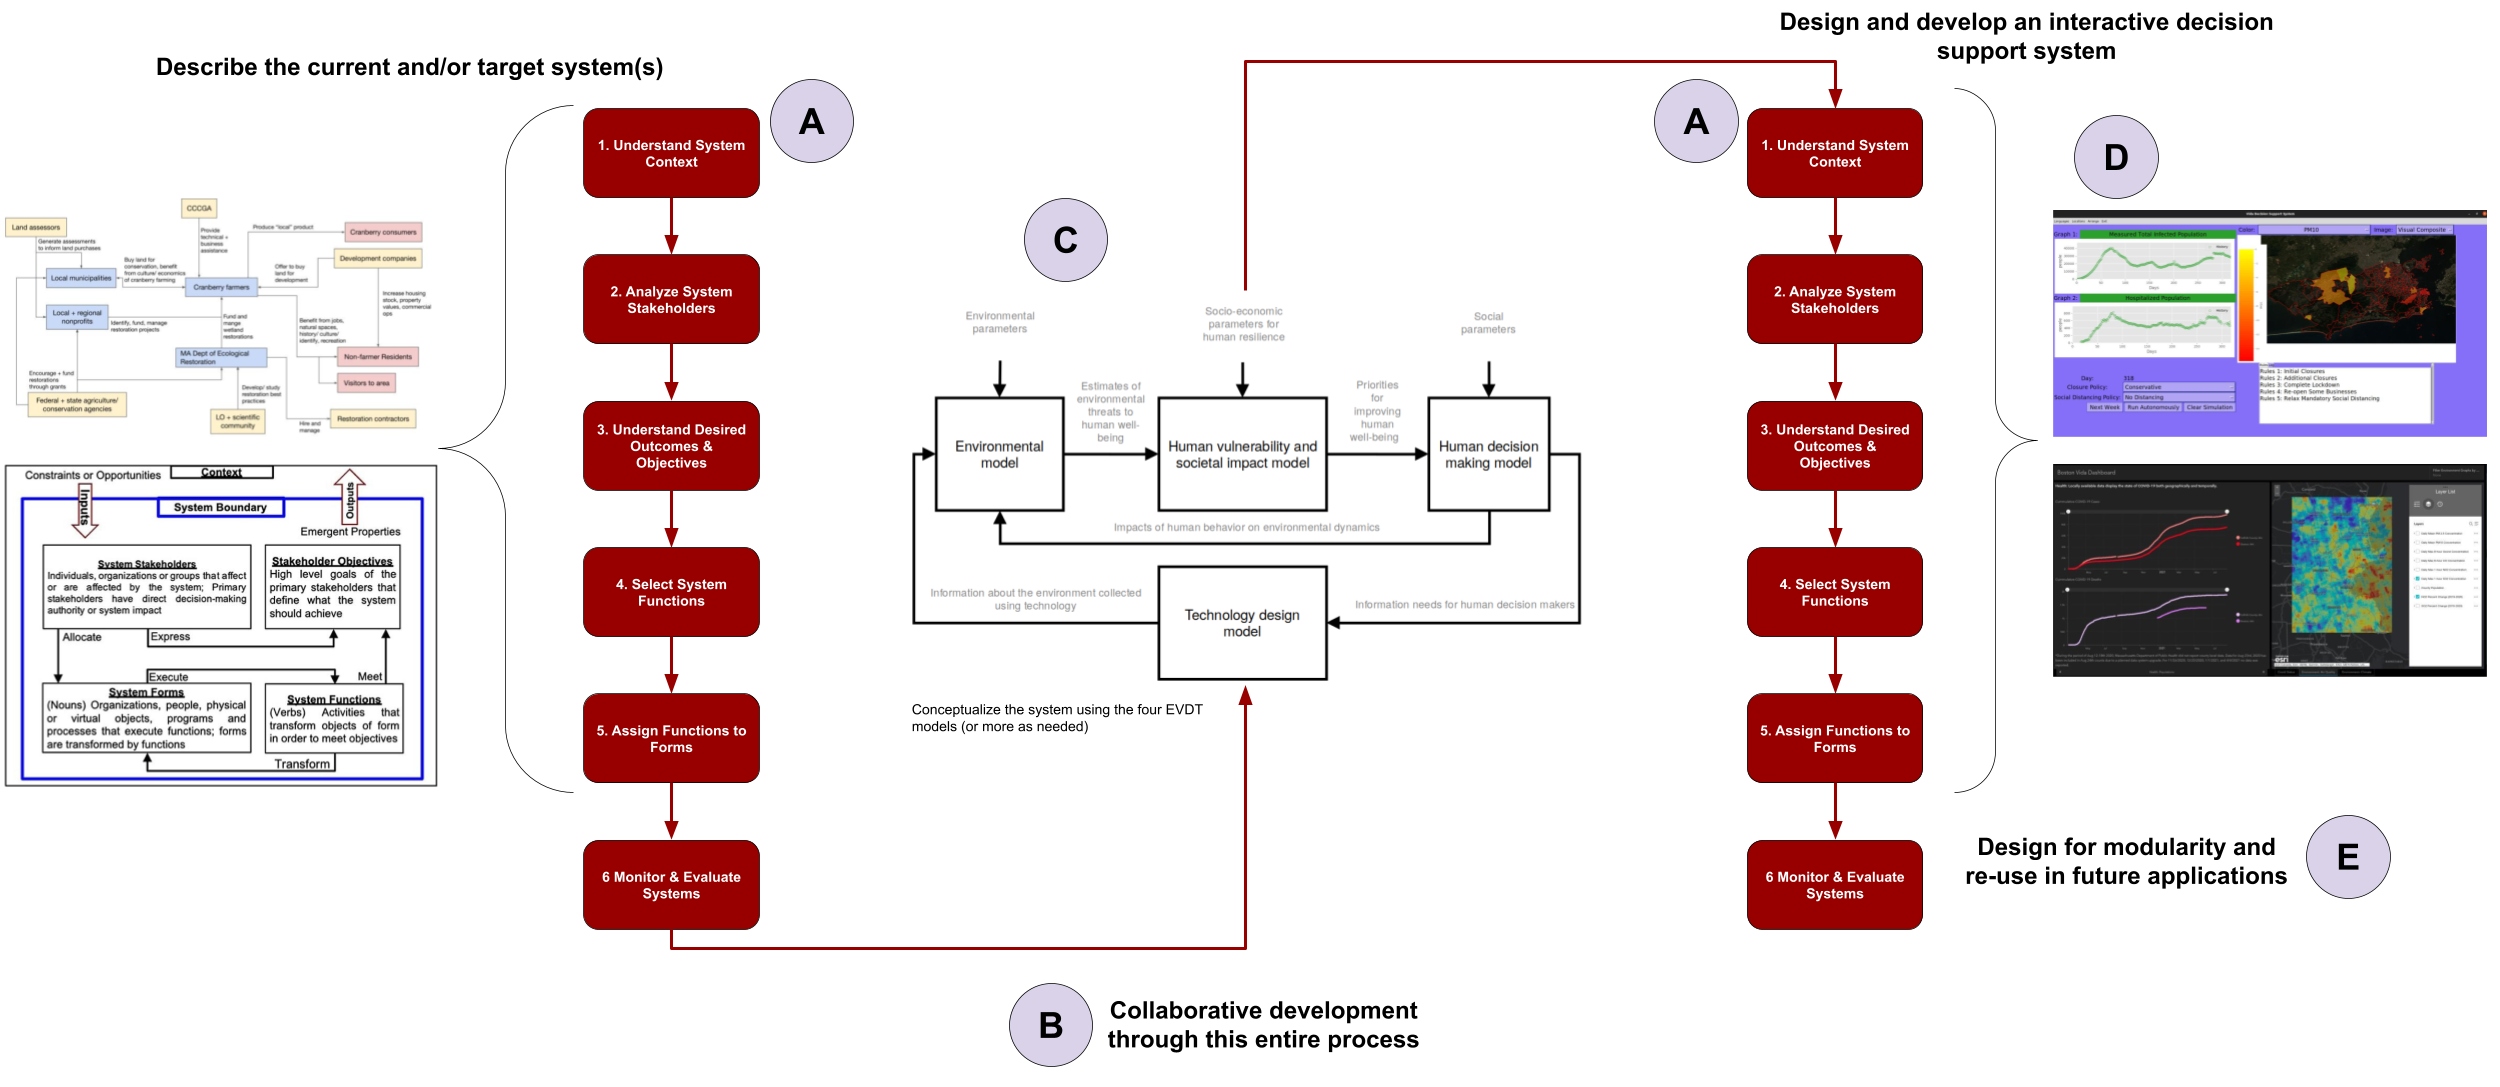
\includegraphics[scale=0.225]{Figures/chap3/evdt_framework_v2.png}
	\caption[Overall EVDT Framework]{Overall EVDT Framework. Lettered circles label the components of the framework. A) The iterations of the Systems Architecture Framework; B) Collaborative development; C) the environment-vulnerability-decisionmaking-technology conceptualization; D) the interactive decision support system output; E) Modularity and re-use}
	\label{fig:evdt_framework}
\end{figure}
\end{landscape}

\subsection{\hlc[cyan]{System Architecture Framework}} \label{sec:saf}

The \acf{saf} is the first element of the \ac{evdt} Framework. The \ac{saf} was developed by Danielle Wood and has gone through several revisions and expansions since its inception \cite{woodAnalysisTechnologyTransfer2013, woodApplyingSystemsArchitecture2014, kazanskyCurrentPotentialRole2016}. The version here is based on the most recent version, as seen in Ovienmhada et al. \cite{ovienmhadaInclusiveDesignEarth2021}. The \ac{saf} builds upon prior work in systems engineering, particularly the subdiscipline of systems architecture as laid out by Maier \cite{maierArtSystemsArchitecting2009} and Crawley \cite{crawley2004}. This prior work tended to be nominally application agnostic, but in practice tended to see application in large aerospace and civil engineering projects. \ac{saf} is similarly application agnostic but has seen its primary uses in international collaborations \cite{pfotenhauerArchitectingComplexInternational2016} and sustainable development \cite{ovienmhadaInclusiveDesignEarth2021}. 

It should be noted that the \ac{saf} includes a variety of technical terms that have similar but not identical definitions to their colloquial use. This terms will typically be indicated with capitalization (e.g. System Boundary). Definitions will be supplied at their first occurrence, but are also listed in the glossary found in Appendix \ref{glossary}.

As defined by Maier, \textit{systems architecture} the art and science of creating and building complex systems, and in particular that part of systems development most concerned with scoping, structuring, and certification \cite{maierArtSystemsArchitecting2009}. This tends to refer to the high level form and function of a system, rather than detailed design. Others, such as Crawley prefer to characterize systems architecture as the mapping of Function to Form such that the essential features of the system are represented. System Functions here mean the specific actions or processes that the system performs. System Forms meanwhile refers to the approaches and structures used to enable the Functions (i.e. the physical ``stuff" of the system). The intent of architecture is to reduce ambiguity, employ creativity, and manage complexity \cite{crawleySystemArchitectureStrategy2015}. Arguably this is a more specific formulation of Maier's definition. In general, Space Enabled and I tend to use Crawley's definition, both due to its clarity, and for the various qualitative and quantitative methods that have been developed to work well with this formulation. 

The current version of \ac{saf} involves six steps, shown in Figure \ref{fig:saf}. It seeks to center the full network of stakeholders and invite them into a collaborative development process. By stakeholders, I mean the people, organizations, and communities that either influence the design and operation of the system or are impacted by the system, or as NASA defines the term: those who are affected by or accountable for an undertaking \cite{nasaofficeofthechiefengineerNASASystemsEngineering2004}. 

\begin{figure}[h] 
\centering
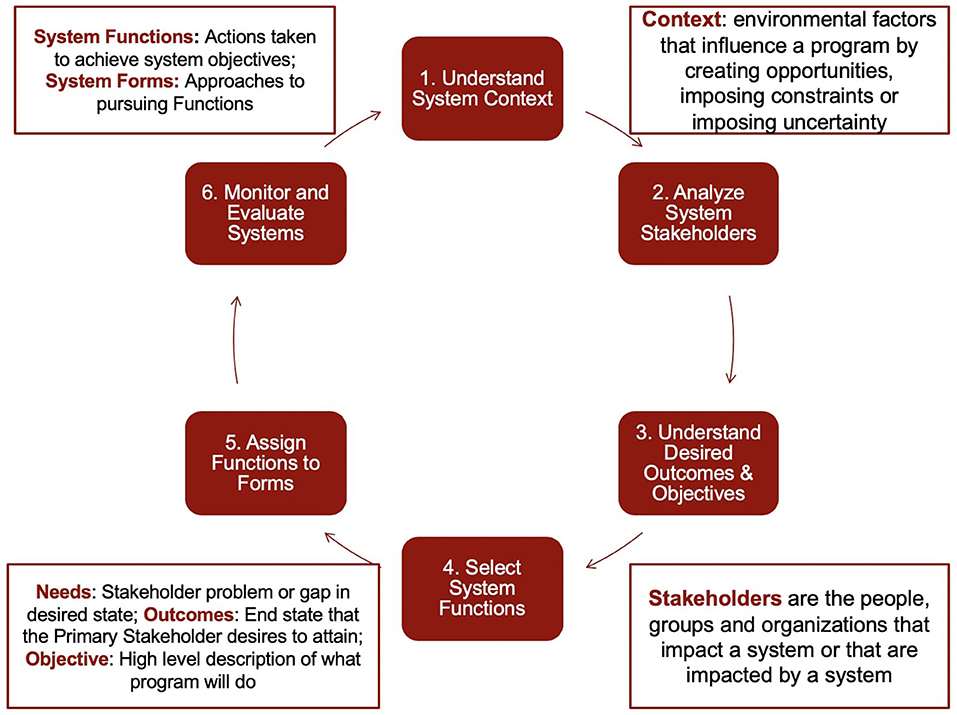
\includegraphics[width=0.9\textwidth]{Figures/chap3/SAF.jpg}
\caption[Six steps of SAF]{Six steps of \ac{saf}.}
\label{fig:saf}
\end{figure}

The primary benefit of a systems architecture approach such as \ac{saf} is, as Crawley articulates
\cite{crawley2004}:

\begin{enumerate}[itemsep=0pt,parsep=0pt]
	\item{Architecture is a way to understand complex systems.}
	\item{Architecture is a way to design complex systems}
	\item{Architecture is a way to design standards and protocols to guide the evolution of long-lived systems.}
	\item{Architecture is a way to manage complex systems.}
\end{enumerate}

As discussed in Sections \ref{sec:se} and \ref{sec:se_critique}, traditionally systems engineering focused on a single stakeholder: the client, with the benefits accruing to that stakeholder primarily. More recent approaches, such as \ac{saf}, expand this to considering the perspectives of multiple stakeholders, though still primarily only using stakeholder input to inform system requirements the beginning of the development cycle. Even \ac{saf} though only explicitly requires the involvement of a wide set of stakeholders during Steps 1-3. If we desire the benefits of a system to not just accrue to central authorities or technocrats but rather to be held by the community themselves, we must ensure keep stakeholders involved through the full cycle.

The following subsections walk through the \ac{saf} steps individually, providing potential methods to achieve each step and discussing continued stakeholder involvement. Section \ref{sec:evdt-collab} will expand how to ensure collaboration and participation throughout the process as well.

A summary of useful methods for each step of \ac{saf} is available in Table \ref{tab:saf_methods}. It should be noted that many of these methods are useful in multiple steps but are listed here in the step that they are primarily associated with. Not all methods are recommended for every application. 

\begin{table}[H]
\caption[Methods for SAF Steps]{Methods for SAF Steps.}
\label{tab:saf_methods}
\begin{center}
\begin{tabular}{ C{4cm} |  L{10cm} } \hline

\textbf{SAF Step} & \textbf{Useful Methods}  \\ \hlinewd{2pt}

\multirow{6}{4cm}{\centering \textbf{1.} Understand System Context} & - Academic literature survey \\
& - Survey of newspapers, periodicals, popular media, and local museums \\ 
& - Informal conversations with stakeholders \\
& - Stakeholder interviews \\
& - Stakeholder surveys \\
& - Direct observation \\ \hline

\multirow{4}{4cm}{\centering \textbf{2.} Analyze System Stakeholders} & Primary-Secondary-Tertiary Classification \\
& - Flowchart relational mapping \\
& - Stakeholder Value Network Analysis \\
& - Agent-based modeling \\ \hline

\multirow{3}{4cm}{\centering \textbf{3.} Understand Desired Outcomes \& Objectives} & Unified objective function and constraints \\
& Monetary conversions (e.g. ecosystem services) \\
& Multi-stakeholder negotiations \\ \hline

\multirow{3}{4cm}{\centering \textbf{4.} Select System Functions \& Objectives} & Multicriteria negotiations \\
& Pairwise comparisons \\
& Delphi method \\ \hline

\multirow{4}{4cm}{\centering \textbf{5.} Assign Functions to Forms}
& System diagramming \\
& Scenario planning workshops \\
& Multi-stakeholder tradespace exploration \\
& Collaborative sketch planning \\ \hline

\multirow{2}{4cm}{\centering \textbf{6.} Monitor and Evaluate Systems}
& Retrospective evaluations \\
& Stakeholder surveys \\ \hline

\end{tabular}
\end{center}
\end{table}

%% \parbox{1\linewidth}{\vspace{0.2cm} 

\subsubsection{\hlc[cyan]{Understand System Context}} \label{sec:saf_context}

The first step of \ac{saf} is to understand the System Context: the external factors that influence and constrain the system. This includes learning about the history of the environments, communities, and organizations that intersect with the system. This information can be of multiple temporal or spatial scales (eg. local, provincial, or international). This step has multiple objectives. The first is to refine the System Boundary: the limit demarcating the system of interest from the rest of the universe. The System Boundary determines what is considered part of the system (and thus subject to the decisions of the designer and stakeholders) and what is not (and is thus considered beyond their control, for the purposes of this project at least). It should be set narrowly enough to provide some level of tractability to both the designer and the major stakeholders, but not so narrowly as to unduly exclude potential interventions from consideration. The designer almost certainly will already have some preconceived System Boundary in mind when starting the project. This step provides a key opportunity to revise that conception, potentially dramatically. Another objective of this step is to identify the stakeholders in the system of interest. This list need not be definitive or exhaustive, as it will be revisited in the next step. Finally, an understanding of the system Context will also inform the feasibility assessment of various system Forms later in the \ac{saf} process.

Methodologies for this step include surveys of literature (including both academic and non-academic literature, including popular media as needed), informal conversations, interviews, surveys, and observation. 


\subsubsection{\hlc[cyan]{Analyze System Stakeholders}} \label{sec:saf_stakeholders}

During the second \ac{saf} step, the various stakeholders, along with the relationships between them, are analyzed. This process may result in the identification of additional stakeholders or the decision to exclude stakeholders from consideration, though the latter should not be done lightly. The primary objectives of this step are (1) to understand how best to engage the stakeholders throughout the rest of the \ac{saf} and \ac{evdt} process; and (2) gain an understanding of how the Stakeholder Needs and Desired Outcomes overlap or conflict. The latter will be further examined in the next step.

A common initial approach for this step is to separate stakeholders into three categories: Primary, Secondary, and Tertiary. This approach, which draws on Crawley et al. \cite{crawleySystemArchitectureStrategy2015} and refined by Wood et al \cite{ovienmhadaInclusiveDesignEarth2021}, defines Primary Stakeholders as those who make direct decision on the design or operation of the system. Secondary Stakeholders are those who have direct influence on the Primary Stakeholders, typically via authority or funding. Tertiary Stakeholders are those that exert either little control or primarily indirect control on the system, but ae impacted by the system. These are somewhat reductive categories and the listing of primary-secondary-tertiary should not be taken to understand a hierarchy of stakeholder worth or importance.

Other methods include both qualitative approaches such as flowchart creation or mapping, and more quantitative approaches such as Stakeholder Value Network Analysis \cite{fengDependencyStructureMatrix2010a} or agent-based modeling. The last of these is more relevant once Stakeholder Needs and Desired Outcomes have been identified. An example of stakeholder relational mapping can be seen in Figure \ref{fig:jaffe-stakeholder}. In its current form, it provided an excellent qualitative aid to understanding stakeholder relations, but it could also have been extended into a more quantitative Stakeholder Value Network Analysis if that had been considered useful.

\begin{figure}[H] 
\centering
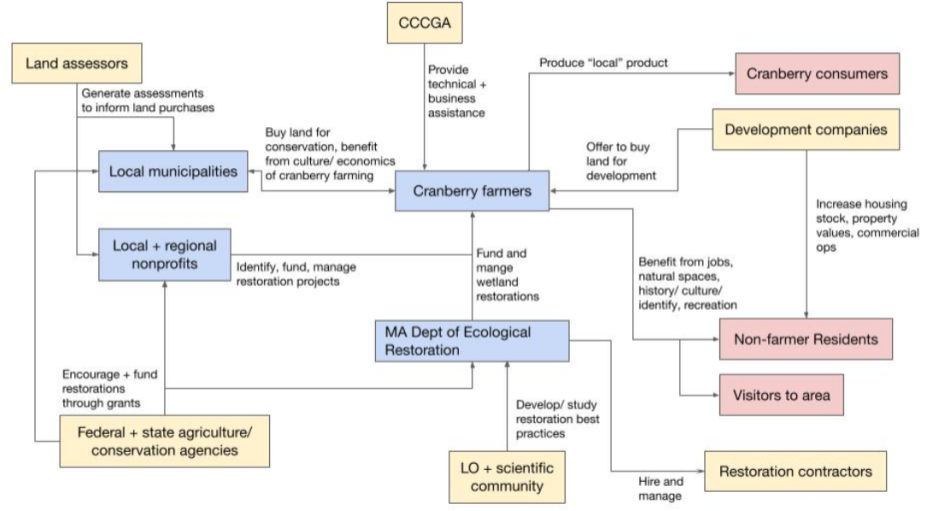
\includegraphics[width=0.9\textwidth]{Figures/chap3/jaffe-stakeholder.png}
\caption[Example stakeholder map of the Massachusetts Cranberry Industry]{Example stakeholder map of the Massachusetts Cranberry Industry. Figure from \cite{jaffeEnvironmentalEconomicSystems2022}}
\label{fig:jaffe-stakeholder}
\end{figure}

\subsubsection{\hlc[cyan]{Understand Desired Outcomes \& Objectives}}

System Needs refer to anything that a stakeholder is lacking. These are not necessarily tied to the system of interest. Desired Outcomes meanwhile are the end states that stakeholder would like to attain. Stakeholder Values are things that stakeholders hold as benefit in relation to needs and desired outcomes. It is important to note that Needs, Desired Outcomes, and Values do not exist in the abstract, but only when tied to a particular stakeholder. This is a critical component of \ac{saf} and one of its major distinguishing characteristics compared to earlier applications of systems engineering to urban planning and development, as discussed at length in Sections \ref{sec:technocracy} and \ref{sec:se_critique}. They will vary from stakeholder to stakeholder, sometimes aligning in constructive ways and sometimes opposing one another. As a result, no singular, objective ``solution" will exist. Tradeoffs will need to be made and the system will serve the interests of some stakeholders more than others. The designer should be aware of this and honest about it. The goal of this step is to synthesize these Needs, Desired Outcomes, and Values, into System Objectives: the high level description of what the system will do.

The methods described in the previous step for understanding relationships between stakeholders are also useful here to see how their needs, desires, and values overlap.

There are at least two schools of thought about how to approach balancing the needs of multiple stakeholders. One school argues for aggregating needs, values, and constraints into a singular objective function and set of constraints prior to considering any particular system functions or forms \cite{hazelriggFundamentalsDecisionMaking2012}. This can be done (a) unilaterally by the designer or a primary stakeholder; (b) through a reduction of all values to a common metric, often monetary; or (c) through a negotiation process among the stakeholders. In general for the kinds of sustainable development applications that \ac{evdt} is envisioned to address, I suggest against this approach. Option (a) is essentially a return to the technocratic hubris criticized in Chapter 2. Option (b) is often difficult and morally problematic. It is difficult because many stakeholder values are difficult to reduce to monetary terms, particularly those values around the natural environment. While the field of ecosystem services (discussed further in Section \ref{sec:rio-vulnerability}) provides some help in this regard, such data is still sparse and unlikely to be comprehensive for a particular application. This option is also morally problematic because reducing values to monetary terms tends to prioritize the needs of wealthy stakeholders (who have more to lose) over economically poorer stakeholders. For example, if a designer is seeking to situate a seawall to reduce damages from cyclones, a purely monetary metric would suggest placing the seawall in front of large vacation homes instead of in front of smaller primary residences. If Option (b) is chosen, I strongly urge the designer to adjust values based on stakeholder wealth to more accurately capture actual impact on the stakeholder. This, of course, adds additional complexity. Option (c) in theory is fine, but many stakeholders will find it difficult to negotiate abstractly, without concrete alternatives available before them. This approach tends to reward those most familiar with fields that deal with the optimization of objective functions, such as systems engineering and economics. By choosing this option, the designer runs the risk of such stakeholders ``gaming the system." This is only worsened by the fact that such stakeholders are disproportionately likely to be in possession of other forms of power and authority.

The second approach is avoid making a unified objective function altogether or at the very least not to set the objective function in stone. Instead various concrete system objectives and form alternatives are proposed to stakeholders and compared in some form of negotiation or voting process. This option is preferred for most \ac{evdt} applications and is discussed further in the following two sections.  

\subsubsection{\hlc[cyan]{Select System Functions}}

During this step, the designer must work with the stakeholder to set System Objectives. These are high level descriptions of what the system must accomplish. They can be quantitative or qualitative. Some sources will use the term System Goals to refer to these to distinguish them from the optimization term ``objective function" \cite{nasaofficeofthechiefengineerNASASystemsEngineering2004}. These objectives will in turn be used to specify System Functions, the actions or processes that the system will perform to accomplish the Objectives.

Multiple techniques are available for coordinating input and involvement from various stakeholders, with varying levels of detail, time requirements, and balance of quantitative versus qualitative information. Examples include  multicriteria negotiations \cite{sparrevikUseMulticriteriaInvolvement2011},  pairwise comparison \cite{motieyanSustainableUrbanPlanning2017}, and various forms of the Delphi method \cite{morganUrbanPlanningUsing1979}. For an excellent survey of multicriteria decision-making analysis methods as applied to sustainable urban planning see Slattery, 2019 \cite{slatteryQuantitativeAssessmentSustainable2019}.

By moving stakeholder negotiations into this step (or even into the following step), the designer is able to provide more concrete examples to stakeholders, reducing the possibility of unforeseen consequences or misstated values. Where time and resources allow, it can be useful to iterate these negotiations at multiple phases: first when selecting System Objectives, again when defining System Functions, and a final time when designing the System Form.

\subsubsection{\hlc[cyan]{Assign Functions to Forms}}

The System Form is what a system is, rather than what it does. The System Form provides the instrument necessary for the System Functions. A particular bicycle is a Form that enables the Function of converting periodic human motion (pedaling) into linear motion (actually going somewhere).

The methods outlined in the previous section are largely still applicable here, as well as some additional approaches that depend on concrete system form alternatives, such as multi-stakeholder tradespace exploration \cite{fitzgeraldRecommendationsFramingMultistakeholder2016} and collaborative sketch planning \cite{vonkSociotechnicalPSSDevelopment2010}. When the system or system intervention is primarily a matter of a policy action, scenario planning workshops can be quite helpful for facilitating the expression of stakeholder preferences or even inducing stakeholders to generate new System Form proposals.

We generally recommend that Steps 1 through 5 be summarized in a concrete visual representation such as Figure \ref{fig:system-diagram}. These can be useful in describing the structure and dependencies within the system, as well as distilling the key aspects of the system in an easily understandable fashion.

\begin{figure}[h] 
\centering
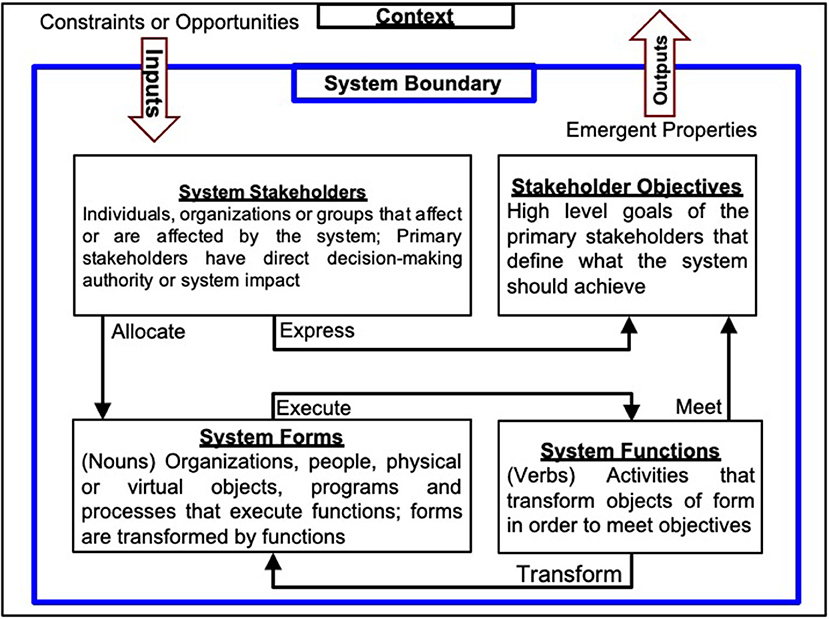
\includegraphics[width=0.9\textwidth]{Figures/chap3/system-diagram.jpg}
\caption[Example system diagram]{Example system diagram. Credit: Danielle Wood}
\label{fig:system-diagram}
\end{figure}

\subsubsection{\hlc[cyan]{Monitor and Evaluate Systems}}

The sixth and final step of \ac{saf} directly leads back to the first. It is a statement that the work is never complete, the system never perfected. Perhaps the system will need to be monitored to ensure that it meets its objectives and further refined if it does not. Perhaps the objectives will change. Or perhaps an additional system needs to be developed to address some of the Stakeholder Needs and Desired Outcomes that went unaddressed in the original process. Either continuous or retrospective evaluations of the system should be conducted. The exact form of these will vary depending on the system at hand but can be as simple as surveying the various stakeholders.

\subsubsection{\hlc[cyan]{A Note on Perspective}}

As implied in the section ``Understand System Context" above, there is a certain level of arbitrariness in defining the System Boundary. This choice affects what stakeholders are included, which stakeholder(s) are made central (if any), and has significant impact on the system objectives, functions, and forms.

When time and resources allow, it can be useful to consider the system from multiple different perspectives before settling on any particular one. As shown in Figure \ref{fig:evdt_framework}, for an application of the \ac{evdt} Framework, I suggest going through the \ac{saf} at twice. The first, Iteration 1, is a purely descriptive process, detailing how the system of interest currently operates.  The second, Iteration 2, which will leverage the above suggested methods more fully, is then used for developing the design of the new system or intervention, be it a product, service, or policy. In projects involving the creation of a \ac{dss} (which \ac{evdt} Framework projects are), the differences between Iteration 1 and Iteration 2 can also help to distinguish the objectives, functions, and form of the \ac{dss} versus the objectives, forms, and functions of the system that the \ac{dss} is supporting decisions about.

It can also be worthwhile to conduct a separate iteration of the \ac{saf} between Iterations 1 and 2 (call this Iteration 1.5). In this iteration, situate the designer or the designers organization as the primary stakeholder. In the case of this thesis, that would be Space Enabled and/or myself. This allows the designer to clearly identify their own personal interests and objectives in the project, rather than to pretend they are a purely altruistic agent (which is rarely the case).
By comparing the results of Iteration 1 and Iteration 2 with Iteration 1.5, the designer can assess whether or not this project is a good fit for them. If their own Needs and Desired Outcomes differ too greatly from those of the other stakeholders, it may be best to not pursue the project. See Section \ref{sec:se_critique} for further discussion of what can occur when a system designer's personal research goals take priority over those of the other stakeholders.


\subsection{\hlc[yellow]{Collaborative Development}} \label{sec:evdt-collab}

Involving stakeholders in the development process, in addition to the requirements definition process, is key for ensuring adoption and capacity building. This has been recognized by the \ac{pgis} movement, which increasingly emphasizes the importance of open source software \cite{williamsonTheirworkDevelopmentSustainable2011, dodgeMappingModesMethods2011}. It is also core to the Data Action framework which, responding to the idea that "data is never raw, it's collected," emphasizes the use of participatory and collaborative methods for collecting and using data \cite{williamsDataActionUsing2020}. Collaborative development is increasingly feasible as barriers have dropped over the past couple of decades. Knowledge and familiarity with computers and programs has expanded, access to sufficient hardware is increasingly common (particularly with the rise of cloud computing platforms), and both synchronous and asynchronous online collaboration tools have proliferated. Obviously such barriers have not been universally eliminated. Furthermore, even in the absence of barriers, not everyone desires to be a computer programmer, earth scientist, \ac{eo} specialist, or social scientist, even part-time. Collaborative development must therefore take different forms in each project, being as welcome as possible to all while accommodating stakeholder preferences and constraints.

\subsection{\hlc[cyan]{EVDT Questions \& Models}} 

The \ac{evdt} Framework conceptualizes the application system from two different perspectives. The first is the system boundaries and stakeholders perspective from \ac{saf} shown in Figure \ref{fig:saf}. The second perspective focuses on combining the established fields of sociotechnical systems \cite{rouseUnderstandingChangeComplex2012,siddiqiSociotechnicalSystemsSustainability2017,sussmanTeachingComplexSociotechnical2010} and socio-environmental systems \cite{elsawahEightGrandChallenges2020} into \ac{sets}. To accomplish this, at least four components are considered: the Environment (data including Landsat, Sentinel, VIIRs, in-situ environmental data and knowledge, etc.); Human Vulnerability and Societal Impact (data including census and survey-based demographic data, eocsystem services valuations, NASA's Socioeconomic Data and Applications Center, local knowledge of impacts, etc.); Human Behavior and Decision-Making (data including policy histories, mobility data, urban nightlight data, community input, etc.); and Technology Design for earth observation systems including satellites, airborne platforms and in-situ sensors (data including design parameter vectors for such systems). The data from each of these domains is used by established models in each domain, which are adapted to work in concert to address the needs identified during the stakeholder analysis. These four components, shown in Figure \ref{fig:model}, seek to encapsulate the major interacting aspects of sustainable development and consider them from a \ac{sets} perspective. 

We are far from the first to argue that such integration is necessary, nor to recognize that it is easier said than done. The closest attempt to what is proposed here is probably that of Shahumyan and Moeckel, though their approach focused on linking together existing models in a loose manner using ArcGIS Model Builder, to avoid having to gain access to proprietary source code. While their example focused on combining transportation, land use, mobile emissions, building emissions, and land cover, with only limited feedbacks, their approach could be extended to capture the full feedback loops proposed by \ac{evdt}. Their example is also proof that the kind of loose integration of library of models that \ac{evdt} envisions is possible \cite{shahumyanIntegrationLandUse2017}. 

The motivation for combining so many variables from different disciplines stems from both push and pull factors. The push factors are the simple increase in availability of data, along with the increase in the interoperability of the variables (which this work itself is trying to contribute to). The primary pull factor is our increased understanding of - and appreciation for - the complex relationships between these domains, relationships that were previously ignored in analyses \cite{gaheganMultivariateGeovisualization2007}. 

\begin{figure}[h]
    \centering
    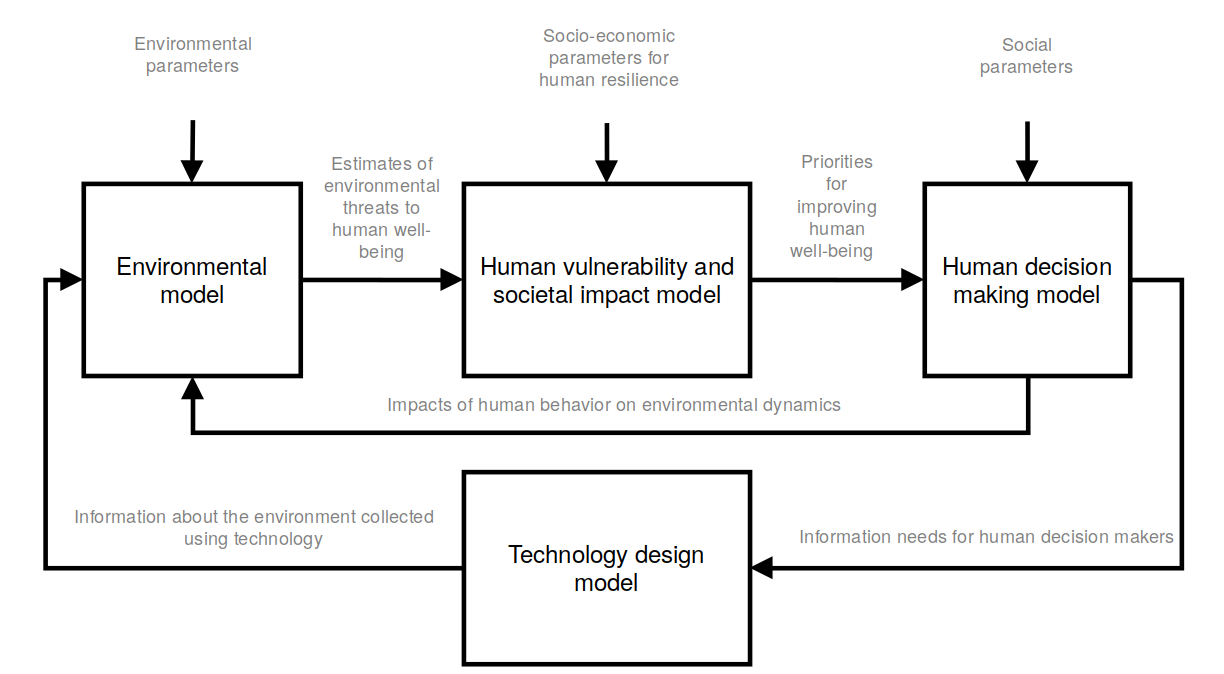
\includegraphics[scale=0.3]{Figures/chap3/modelflow.png}
    \caption[Generic version of EVDT Model] {Generic version of the Environment - Vulnerability - Decision - Technology Model}
    \label{fig:model}
\end{figure}

This set of four models with the particular linkages shown in Figure \ref{fig:model} are not the only form that \ac{evdt} can take, merely the most general arrangement. Some applications may involve replacing a model with a human-in-the-loop (e.g. having the user themself substitute for the decision-making model) or omitting a model altogether. For other applications, it may make sense to conceptually break a model into two or more components. In the Vida project, it was considered worthwhile to separate the social impact model into two components, one focusing on public health (the obvious priority when dealing with COVID-19) and one focusing on non-health metrics (such as income, employment, etc.). Such a separation can be useful if either significantly different modeling methodologies are going to be used or if the linkages with the other \ac{evdt} components are different from one another. 

One way to determine the optimal arrangment of \ac{evdt} components is to consider what questions the user or researcher is seeking to answer with this application of \ac{evdt}. For instance, the default \ac{evdt} arrangement shown in Figure \ref{fig:model} was motivated primarily by the following four questions:

\begin{enumerate} \setlength{\itemsep}{0pt} \setlength{\parskip}{0pt}
    \item What is happening in the natural environment?
    \item How will humans be impacted by what is happening in the natural environment?
    \item What decisions are humans making in response to environmental factors and why?
    \item What technology system can be designed to provide high quality information that supports human decision making?
\end{enumerate}

Alternate questions may result in a different configuration or set of components (further discussion of this in Section \ref{sec:intended}). The point of \ac{evdt} is not to insist upon a particular set of linkages and feedbacks, but rather to encourage a consideration of such linkages between domains in general, and to consider them through a systems engineering perspective. Of course answering the structuring questions, and even phrasing them in the first place, requires the use of collaborations.

\subsection{\hlc[yellow]{Interactive Decision Support System}} 

A key aspect of the term \ac{dss} is the word "support." Crawley et al. state that the goal of a \ac{dss} is to "\emph{enhance} the efficiency of decision makers by providing tools to quantitatively and qualitatively explore a space of alternatives for single or multiple decisions" [emphasis added] \cite{crawleySystemArchitectureStrategy2015}. This means that the \ac{evdt}-developed \ac{dss} should not present decisions as a \textit{fait accompli} but instead support stakeholders in developing their own solutions. Ideally this means that individual stakeholders can directly handle and explore any simulations or models used, along with their underlying assumptions and structure. If this is not feasible, an indirect form of interaction can be used, such as when a stakeholder provides verbal instruction to someone who then implements that instruction in the \ac{dss}. The latter option can be quite useful when there are barriers of language, familiarity, or technical knowledge, and is commonly used in purposeful gaming \cite{rossGamebasedLearningSystems2014}, wargaming \cite{hansonImprovingOperationalWargaming2016,selvaRevitalizingWargamingNecessary15,shlapakReinforcingDeterrenceNATO2016}, and role playing gaming \cite{groganStrategicEngineeringGaming2012,groganFederatedSimulationGaming2012}. Additionally, in contrast to Crawley's definition which centers on the "efficiency of decision-makers," we argue that an ideal \ac{dss} should cause a decision-maker to consider multiple perspectives (such as the four models of \ac{evdt} and those of other stakeholders) and thereby make \textit{better} decisions as well.

\subsection{\hlc[yellow]{Re-use \& Community Development}} 

One of the key motivations of participatory, stakeholder-involved processes is capacity building. In the case of the \ac{evdt} Framework, this includes both capacity building in a specific application community and in the broader practitioner community of those using \ac{eo}, \ac{gis}, and systems engineering for sustainable development. To that end, the \ac{dss} should be designed with re-use and modularity in mind. The ability to track mangrove health in Brazil \cite{reidInteractiveModelAssessing2020} proved to be useful in a later application in Indonesia \cite{lombardoEnvironmentVulnerabilityDecisionTechnologyFrameworkDecision2022}. A key aspect of this is making as much of the \ac{dss} code available in open source repositories.

The second form of capacity building is pursued by developing a community of practice around \ac{evdt} and related endeavors.

\section{\hlc[cyan]{Intended Applications \& User Types}} \label{sec:intended}

\ac{evdt} is not intended to be an exclusive project of Space Enabled. It also not intended to be a framework used by isolated individuals. We actively invite involvement from other systems engineers and those from other disciplines. Through this proposed thesis and other related projects, the framework will be refined, initial applications demonstrated, a basis of code built (already available online \cite{bluerasterBlueRasterVida2021,reidEVDTRepository2020,reidMITVidaRepository2021}), and a community of collaboration sprouted. These will can be built upon for building a community of practice, where individuals can contribute in a variety of ways, as shown in Figure \ref{fig:development}.

\begin{figure}[h]
	\centering
	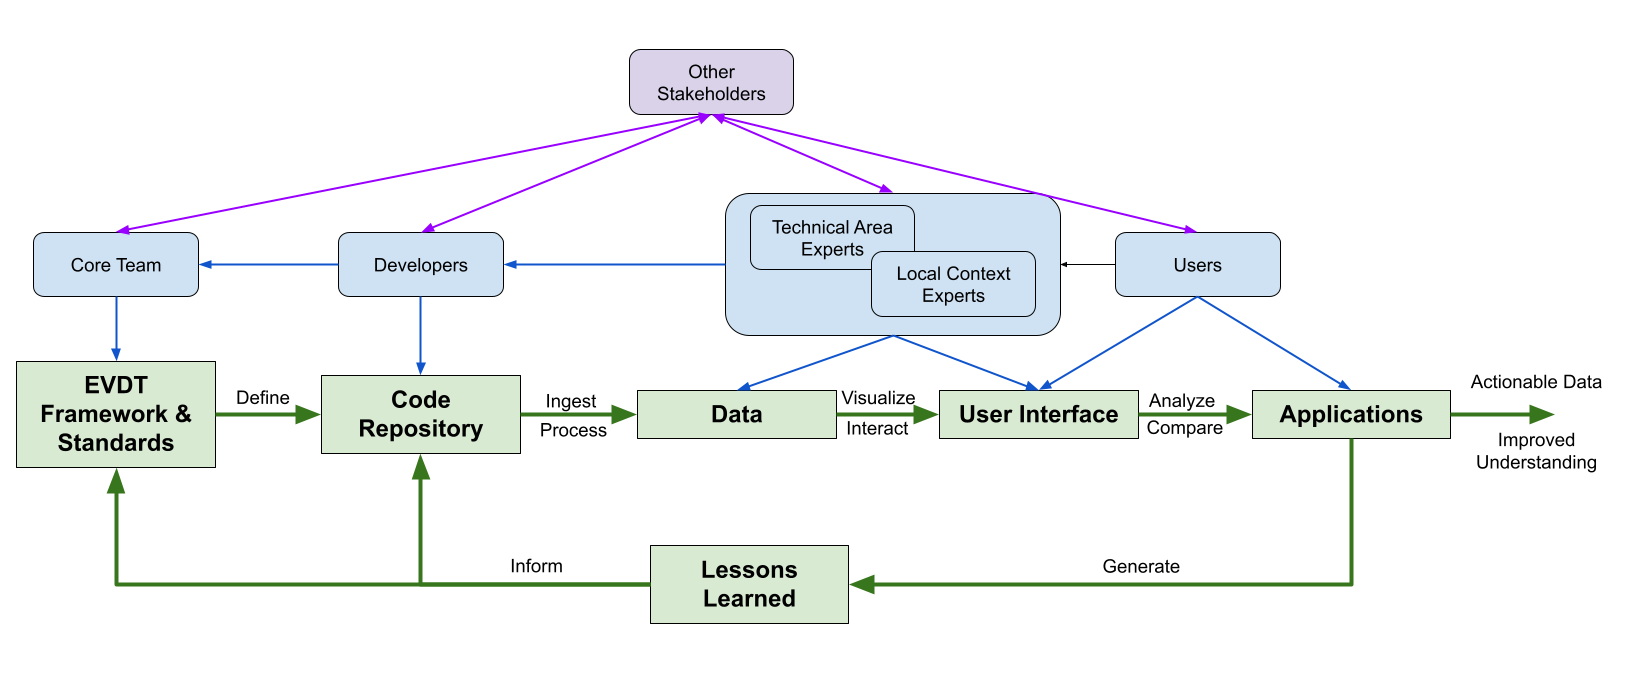
\includegraphics[scale=0.25]{Figures/chap3/Graphic_2_Development.png}
	\caption[The EVDT development pipeline] {The EVDT development pipeline. Note that the different community groups, shown in blue, are not necessarily discrete and one individual could simultaneously participate in multiple.}
	\label{fig:development}
\end{figure}

It is worth further describing some of the categories of \ac{evdt} community members shown in the blue boxes of Figure \ref{fig:development}. What follows will be a generalized discussion of these categories. Specific instances for this thesis are discussed in Chapters \ref{ch:mangroves} and \ref{ch:vida}.

Moving from left to right, the \textit{Core Team} refers to those directly involved in the development of the \ac{evdt} Framework. Right now this is essentially a set of researchers in Space Enabled and some close academic affiliates. This team is likely to remain predominently academic moving forward, though could transition to involving individuals or organizations from \acp{ngo} in the future. The members of this team will typically have expertise with sustainable development and \acp{dss}, significant experience with \ac{evdt}, and investment in its success. Particularly once \ac{evdt} is more developed, this core team is likely to be formally defined.

The \textit{Developers} includes all those who actively develop the models, user interfaces, visualizations, and other associated aspects of the \ac{dss} software for the various \ac{evdt} projects. These will typically be individuals with expertise in \ac{gis}, coding, and/or data processing. Thus they are likely to work in academia or as analysts in a government agency or \ac{ngo}, though the project will be open source, membership in this category will not be formally defined and participation will be encouraged at any level of expertise or degree of involvement. Currently the Developer team is largely the same as the Core Team, though we have some developer involvement from other collaborators as well.

\textit{Technical Area Experts} refers to experts in some relevant domain to an \ac{evdt} project but are consulted but not directly involved in the ongoing development of the \ac{evdt} Framework and code repository. This could include individuals such as ecosystem services economists, human mobility researchers, or fisheries experts. They will typically come from the ranks of academia, though it is not unreasonable to expect some number of government analysts or \ac{ngo} researchers.

\textit{Local Context Experts} refers to those who have a high level of knowledge of the \ac{sets} and stakeholders of a particular \ac{evdt} project. This could include a local community leader, an experienced activist, or a local government official. This category is grouped together with \textit{Technical Area Experts} as the line between the two is oftentimes blurry. A local university researcher who studies the economics of informal housing and who specializes in the city involved with a particular \ac{evdt} project is arguably both a Technical Area Expert and a Local Context Expert.

\textit{Users} refers to those who directly use the \ac{dss} software developed through an \ac{evdt} project. Exactly who these are will depend on the specific project and thus their level of experience with mapping, earth science, or development may vary significantly. They should be direct stakeholders in the specific \ac{evdt} project and have some involvement with the decision-making process (though not necessarily formal involvement). 

It should also be emphasized that while Figure \ref{fig:development} is fairly linear, the \ac{evdt} Framework emphasizes collaborative development. One person may serve multiple roles in the pipeline and, even if not, stakeholders, including users, should be involved throughout the \ac{dss} development process.

As the number of applications increase and the code is refined, the various models used in the applications may themselves be the first members of an openly accessible library of models. Potential user groups could adapt and reuse \ac{evdt} components in other applications, without having to start from scratch. Initially this would likely still require significant code expertise, but it is entirely possible for functionality to be created to allow for `plug-and-play.' A user may be able to, in browser or on desktop, select a geographic area of interest (e.g. the Sóc Trăng Province of Vietnam), select an environmental model (e.g. coastal forest health), a societal impact model (e.g. cyclone vulnerability), a decision-making model (land use conversion and conservation policy), and a technology model (satellite versus in-situ monitoring), all without writing a line of code (though perhaps being required to import new datasets themselves). Such functionality, along with the recruitment pipeline shown in Figure \ref{fig:development}, help to expand participation in all aspects of \ac{evdt}. In this way the user base will be expanded beyond initially invested experts.

We are cognizant that making \ac{evdt} truly participatory is easier said than done, but we do believe it is a worthy goal. In addition to model interoperability standardization, the code moderators will need to specify accessibility norms as well, so as to ensure usability by individuals with a wide range of backgrounds. Existing prototypes have made some steps in this direction, by having multiple language options available. Thus far, this has been accomplished by existing language knowledge of code moderators as well as the occasional volunteer translator, but some more targeted efforts may be required in the future to specifically recruit translators for targeted languages.

Language is not the only accessibility barrier, however. Terminology, presentation, and interactiveness can also be differentiately accessible to different individuals, depending factors such as educational or cultural background. That said, these difficulties can be addressed via some of the same methods that are already core to the \ac{evdt} methodology: namely partnerships with local collaborators; stakeholder analysis; and iterative, participative design. 

Another consideration in the future of \ac{evdt} are the types of applications that it will be used for. Some potential applications include:

\begin{enumerate} \setlength{\itemsep}{0pt} \setlength{\parskip}{0pt}
    \item To inform sustainable development policies. Ex) Comparing the impact of different conservation and zoning policies on the local environment and on economic outcomes.  \label{item:policy}
    \item To educate on the connections between the different \ac{evdt} domains. Ex) Demonstrating the local ecosystem services value of treecover in an urban environment.
	\item To facilitate the comparison of different remote sensing data products for particular applications. Ex) Considering whether to commission periodic aerial surveys of an area or to rely on "free" civil satellite data, such as Landsat and Sentinel. \label{item:data}.
    \item To facilitate the exploration and evaluation of new sensing technology architectures for particular applications. Ex) Designing a new \ac{lidar} satellite to assist forest management in a particular region. \label{item:tech}
    \item To facilitate scientific research on ecosystem services and/or the impacts of human behavior on the environment. Ex) Simulating different casual connections and comparing the simulated data with historical data, to assess the strength of those connections.
    \item To provide a basis for studies of the effectiveness of different \ac{dss} attributes. Ex) Assessing visualization techniques, workshop formats, etc. \label{item:user}
\end{enumerate}

These applications are varying levels of interest and importance to different stakeholders, and some could potentially be viewed as competing for development resources and focus. In some cases they may rely upon different configurations of the \ac{evdt} components, as shown in Figure \ref{fig:combo}. For instance Items \ref{item:data} and \ref{item:tech} (best served by configuration B of Figure \ref{fig:combo}) require a functional model of the relationships between different remote observation design parameters and performance parameters, along with a means of visualizing and exploring the tradespace (as has been proposed by Siddiqi et al. \cite{siddiqiValuingNewEarth2019}). A user who is predominantly interested in Item \ref{item:policy} (configuration A) may find this functionality irrelevant or outright distracting.

On the other hand, some applications are more complementary. While the Item \ref{item:policy} is likely to be a government official or community member while the Item \ref{item:user} user is likely to be an academic researcher, the findings from Item \ref{item:user} would result in the design of \ac{evdt} being improved, so as better serve the needs of the Item \ref{item:policy} user.

Ideally, \ac{evdt} would be open to all these applications and more. In practice, care must be taken so that interests of one user group do not unintentionally dominate those of others or, worse, that the interests of the developers do not send them on a path counter to the interests of the users. This will thus require ongoing discussion and consideration with the \ac{evdt} community.

It should also be recognized that not all users will engage with the \ac{evdt} \ac{dss} software products directly or in the same way. As shown in Figure \ref{fig:development}, some stakeholders and community members will participate in the \ac{saf} process, but may not directly interact with the \ac{evdt} software products themselves. This is both due to the fact that many people are unlikely to have the time or inclination to do so (understandably so) and due to various barriers that will doubtlessly remain despite the efforts of \ac{evdt} developers. Such barriers include access to the internet, computing power, and electricity. While all of these are becoming available to an increasing number of people globally, they are by no means ubiquitous. Initial prototypes have \ac{evdt} have pursued both offline, desktop version and online, browser-based versions to try and accomodate different levels of resource access. Such issues will need to be considered as part of future development decisions as well.

Finally, this envisioned development and expansion process is fundamentally a "snowball model." Existing team members collaborate with new partners and their communities. This results in additional team members who can then collaborate with others. \ac{evdt} may (and should aim) to one day be easily accessible even in the absence of connections to existing community members, but that is not in the immediate future.

\clearpage
\begin{figure}[h]
	\centering
	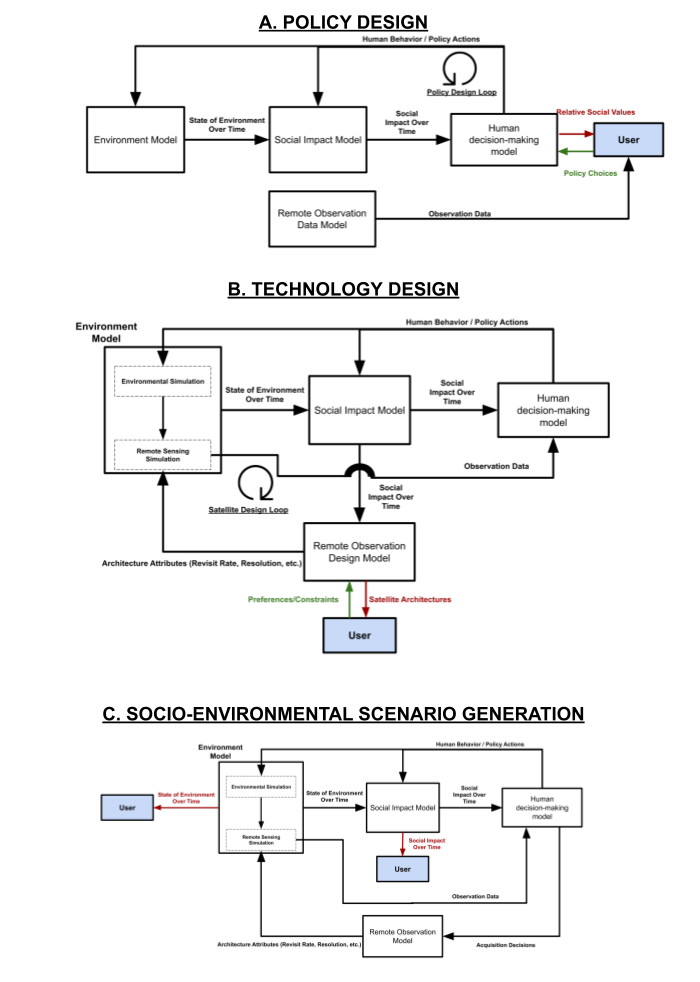
\includegraphics[scale=0.5]{Figures/chap3/Loops_Combined.png}
	\caption{Three example EVDT research configurations}
	\label{fig:combo}
\end{figure}
\clearpage

\section{\hlc[cyan]{Novelty of EVDT}} \label{sec:novelty}

It is important to establish what aspects of \ac{evdt} are novel and how this framework relates to the current state of practice. 

Computational models have long been closely linked to the pursuit of sustainable development and with its definition, stemming from the World3 system dynamics model underlying the Club of Rome's \textit{The Limits to Growth} report in 1972 \cite{meadowsLimitsGrowth1972}. As was discussed in Section \ref{sec:se}, the development field would largely come to repudiate such efforts in the mid-to-late 1970s, only to come back around to modeling on their own terms in the subsequent decades. Thus it cannot be said that \ac{evdt} is new in saying that modeling plays an important role in sustainable development. 

Nor can it be said that \ac{evdt} is the first to advance the concept of multidisciplinary, integrated models in development applications. To refer to just a handful of examples:

\begin{itemize} \setlength{\itemsep}{0pt} \setlength{\parskip}{0pt}
	\item{The open source UrbanSim combines land use, transportation, and certain environmental factors in a dynamic, area-based simulation system that, similar to \ac{evdt}, is a collection of multiple models \cite{waddellUrbanSimModelingUrban2002}.}
	\item{The agent-based \ac{ilute} model simulated the urban spatial form, demographics, travel behavior, and environmental impacts for the Toronto area \cite{millerHistoricalValidationIntegrated2011}.}
	\item{The TripEnergy model combines an environmental submodel (transportation systems) and societal impact submodel (energy consumption and emissions of vehicles) \cite{needellEfficientlySimulatingPersonal2018}. It is then combined with a model of human decision-making to create Tripod, "a smartphone-based system to influence individual real-time travel decisions by offering information and incentives to optimize system-wide energy performance" \cite{azevedoTripodSustainableTravel2018}.}
	\item{The closest attempt to what we are proposing here is probably that of Shahumyan and Moeckel, though their approach focused on linking together existing models in a loose manner using ArcGIS Model Builder, to avoid having to gain access to proprietary source code. While their example focused on combinging transportation, land use, mobile emissions, building emissions, and land cover, with only limited feedbacks, their approach could be extended to capture the full feedback loops proposed in \ac{evdt}. Their example is also proof that the kind of loose integration of library of models that \ac{evdt} envisions is possible \cite{shahumyanIntegrationLandUse2017}.}
\end{itemize} 

In the field of earth science, integrated models have also become increasingly common. Originally developed for operational weather forecasting, \acp{osse} have found widespread use for designing earth observation systems at \ac{nasa} and elsewhere \cite{masutaniObservingSystemSimulation2010}, by linking models of environmental phenomena with simulations of observing platforms (both hypothetical and real). These models are rigorously validated \cite{erricoDevelopmentValidationObservingsystem2013} and are often custom-made for a particular mission. Significant progress has been made however by the  Hydrological Sciences Laboratory and Earth Science Technology Office at \ac{nasa} in developing the \ac{lis}, a more reusable and inter-operable modeling tool with numerous earth sciences applications (soil moisture, hydrology, meteorology, etc.) \cite{kumarMissionSimulationEvaluation2015}. One of these uses is the easier development of \acp{osse}, as a means of facilitating technological development. Since the development of the \ac{lis}, the Hydrological Sciences Laboratory has worked to make the earth science models more accurate, utilize  a broader range of computational methods, and standardize the validation and evaluation processes for \acp{osse}.

Systems engineering has also recently seen a handful of approaches proposed for use in sustainable development. In 2020, Honoré-Livermore et al. sought to address the \acp{sdg} in arctic coastal regions via an approach grounded in \ac{ses} and the \ac{spade} methodology \cite{honore-livermoreAddressingSustainableDevelopment2020}. The \ac{spade} methodology was developed specifically for sustainable development applications. The five components of its name constitute five non-linear steps, each of which has various specific associated methodologies \cite{haskinsSystemsEngineeringAnalyzed2008}, as shown in Figure 3.

\begin{figure}[h]
\centering
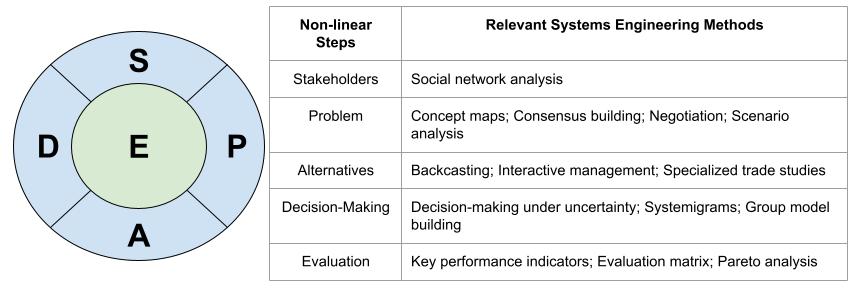
\includegraphics[scale=0.4]{Figures/chap3/spade.png}
\caption[The SPADE Methodology and associated methods]{The Stakeholders-Problem-Alternatives-Decision-Making-Evaluation (SPADE) Methodology and associated methods. Adapted from Haskins, 2008 \cite{haskinsSystemsEngineeringAnalyzed2008} as seen in \cite{reidSystemsEngineeringAppliedPendingPublication}.}
\label{fig:spade}
\end{figure}

Van Zyl and Root meanwhile used a transdisciplinary approach involving Wilbur's integral systems theory \cite{esbjorn-hargensOverviewIntegralTheory2010} and the \ac{catwoe} framework from \ac{ssm} \cite{checklandSoftSystemsMethodology2000} to design sustainable agricultural principles in New Zealand \cite{vanzylTransdisciplinaryDesignImplementation2020}.

Other recent approaches focus on scenario planning and education for understanding evolution of the urban form \cite{geyerSystemsEngineeringMethodology2014}, sustainable land-use planning that relies upon multilevel stakeholder partnerships \cite{puchol-salortUrbanPlanningSustainability2021}, a synthesis of participatory planning with systems engineering for sustainable regional planning \cite{aspenDevelopingParticipatoryPlanning2021}, and leveraging human-centered design to address the \acp{sdg} \cite{muellerUsingHumanCenteredDesign2020}. A survey of sustainable development applications of systems engineering can be found in Yang and Cormican, 2021 \cite{yangCrossoversConnectivitySystems2021}, which itself was published in a special issue of \textit{Sustainability} dedicated to systems engineering \cite{haskinsSystemsEngineeringSustainable2021}.

Common across all of these methods are a significant consideration of a wide set of stakeholders and an adoption of different systems engineering techniques for integrating these stakeholder needs into the system design and development process.

All of this clearly demonstrates that I am far from the first to argue that such multidisciplinary integration is necessary, for the potential utility for systems engineering in sustainable development, nor to recognize that both are easier said than done \cite{shahumyanIntegrationLandUse2017}. What then, does the \ac{evdt} framework specifically have to offer? 

First, there is the developmental process and theoretical underpinnings of \ac{evdt}: the combination of systems architecture (and other systems engineering techniques), \ac{gis}, collaborative planning, and remote observation. As was argued in Chapter \ref{ch:theory}, these fields each of complementary aspects that can be brought to bear in the development of future \acp{dss}.

Second, there are distinct advantages to the development and codification of a concrete framework for such integrated modeling projects for sustainable development applications. Many of the above examples of integrated models were developed either without such a framework at all (a one off model intended to solve a particular problem or demonstrate a particular technique) or for a different class of applications (the \ac{osse} framework is fundamentally about designing better \acp{eos} for scientific purposes). Those few that have both a dedicated framework and a sustainable development focus (this includes \ac{servir}, \ac{fews}, and various \ac{un}-affiliated programs such as the World Food Program) are intended for large governmental (often multi-nation and/or multi-agency) teams and typically are aimed at national or even multinational applications. There is a real need for a framework that is dedicated for sustainable development applications of small scales, accessible to relatively small teams for specific, targeted projects. The \ac{evdt} framework has the potential to fill that gap. Research Question 1 is aimed at developing the \ac{evdt} Framework in detail and identying these advantages. Research Question 2 is then aimed at demonstrating these advantages.

%Miller argues that, despite the historical dificulties that integrated urban models have had, there is reason to be optimistic about the state of the art moving forward, particularly for integrating transportation and land-use models in particular \cite{millerIntegratedUrbanModeling2018}. <---important to discuss at more length

\section{\hlc[red]{Development \& Evaluation}}


\section{\hlc[red]{Mapping and Visualization}}


"A single map is but one of an indefiniteliy large number of maps that might be produced for the same situation or from the same data." \cite{monmonierHowLieMaps1996}

Data maps have a long history. Tufte dates them to the seventeenth century and cites Edmond Halley's 1686 chart of trade winds as "one of the first data maps" \cite{tufteVisualDisplayQuantitative2001} though arguably Scheiner's 1626 sunspot visualization qualifies as a data map \cite{friendlyBriefHistoryData2008}, as perhaps do Polynesian knot maps, which long predates either [CITE]. Graphing data over time, meanwhile dates by to the 14th century \cite{friendlyBriefHistoryData2008}.

Choropleths are one of the more common types of non-imagery geospatial data that \ac{evdt} uses. These are maps that express "quantity in area" (i.e. some statistic tied to a particular geographic area with color, texture, or shading). It should be noted that choropleths have a few well-known limitations, including the ecological fallacy and the modifiable areal unit problem \cite{cramptonRethinkingMapsIdentity2011, sawickiNeighborhoodIndicatorsReview1996}. It is for these reasons that \ac{evdt} does not rely entirely on choropleths and why we strive to store data with the finest geospatial resolution available.

Historically, \ac{gis} implementations have often struggled to handle temporal data \cite{harrisLocationalModelsGeographic1993}.

Historically social indicators tended to be defined for city, province, or national areas, the \acp{mdg} and \acp{sdg} being the preeminent examples of the latter. Advances in \ac{gis}, however did enable the creation of more neighborhood level indicators starting in the late 1990s \cite{sawickiNeighborhoodIndicatorsReview1996}. 

Sawicki and Flynn argue that one must specify the goals before specifying what indicators to use. From their list of possible aims, the following are the most relevant to \ac{evdt} \cite{sawickiNeighborhoodIndicatorsReview1996}:

\begin{itemize}[itemsep=0pt,parsep=0pt]
	\item{Developing dynamic models of neighborhood change}
	\item{Evaluating the likely impact of existing and/or poposed policies on neighborhoods and/or their residents.}
	\item{Measuring inequality over space and time both within and between regions.}
\end{itemize}



Initial versions of \ac{evdt} and Vida featured quite large graphics. Tufte argues that graphics in general should be significantle shrunk and that "many data graphics can be reduced in area to half their current published size with virtually not loss in legibility and information." \cite{tufteVisualDisplayQuantitative2001} Inaccordance with this Shrink Principle, these graphics were greatly reduced in later versions.

As with most \ac{gis} software \cite{heikkilaGISDeadLong1998}, early verions of \ac{evdt} were structured as entirely object-oriented, and later versions remained primarily object-oriented. This has many advantages but also comes at certain costs, the most important of which include (a) difficulty in recording continuous spatial variables and (b) a requirement to pre-identify the different classes (objects) to sort phenomena and relationships into \cite{goodchildModelingEarth2011}. 

It is recognized that this desktop version comes with numerous downsides. \textit{theirwork}, an early collaborative, open source \ac{gis} platform, specifically "decided at an early stage to make the software Web-based to allow for a process of rapid development and iteration and allow a maximum number of potential participants." \cite{williamsonTheirworkDevelopmentSustainable2011} It should be noted, however, that \textit{theirwork} was a UK-based project (an area with high internet connectivity penetration) and started in the mid 2000's, a period with significantly diversity of internet browsing methods, which simplified the task of ensuring accessibility. Nonetheless, it is impossible to deny the collaboration and software sustainability benefits of an online platform, particularly in an age when many of the early concerns with the internet (low speeds, lack of knowledge about how to use it, etc.) \cite{shifterInteractiveMultimediaPlanning1995} have been largly alleviated.

the meeting arrangment that EVDT supports, Table \ref{table:meeting_arrangements}

\begin{table}[h]
\caption[Different types of meeting arrangements]{Different types of meeting arrangements. Adapted from \cite{jankowskiGISGroupDecision2001}}
\label{table:meeting_arrangements}
\begin{center}
\begin{tabular}{ L{3cm} L{5.5cm}  L{5.5cm}}  \hline
 & \textit{Same time} &\textit{Different time}  \\ \cline{2-3}
\textbf{\textit{Same place}} & \textbf{Conventional Meeting} \qquad \textit{Advantage:} 
\vspace{-5mm}
\begin{itemize}
    \setlength{\itemsep}{0pt}%
    \setlength{\parskip}{0pt}%
	\item{face-to-face expressions}
	\item{immediate response}
\end{itemize} &
\textbf{Storyboard meeting} \qquad \textit{Advantage:} 
\vspace{-5mm}
\begin{itemize}
    \setlength{\itemsep}{0pt}%
    \setlength{\parskip}{0pt}%
	\item{scheduling is easy}
	\item{respond anytime}
	\item{leave-behind note}
\end{itemize} 
\\
& \textit{Disadvantage:} 
\vspace{-5mm}
\begin{itemize}
    \setlength{\itemsep}{0pt}%
    \setlength{\parskip}{0pt}%
	\item{scheduling is difficult}
\end{itemize} &
\textit{Disadvantage:} 
\vspace{-5mm}
\begin{itemize}
    \setlength{\itemsep}{0pt}%
    \setlength{\parskip}{0pt}%
	\item{meeting takes longer}
	\item{difficult to maintain in the long run}
\end{itemize} 
\\ \hline

\textbf{\textit{Different place}} & \textbf{Conference call meeting} \qquad \textit{Advantage:} 
\vspace{-5mm}
\begin{itemize}
    \setlength{\itemsep}{0pt}%
    \setlength{\parskip}{0pt}%
	\item{no need to travel}
	\item{immediate response}
\end{itemize} &
\textbf{Distributed meeting} \qquad \textit{Advantage:} 
\vspace{-5mm}
\begin{itemize}
    \setlength{\itemsep}{0pt}%
    \setlength{\parskip}{0pt}%
	\item{scheduling is convenient}
	\item{no need to travel}
	\item{submit response anytime}
\end{itemize} 
\\
& \textit{Disadvantage:} 
\vspace{-5mm}
\begin{itemize}
    \setlength{\itemsep}{0pt}%
    \setlength{\parskip}{0pt}%
	\item{limited personal perspective from participants}
	\item{meeting protocols are difficult to interpret}
	\item{difficult to maintain meeting dynamics}
\end{itemize} &
\textit{Disadvantage:} 
\vspace{-5mm}
\begin{itemize}
    \setlength{\itemsep}{0pt}%
    \setlength{\parskip}{0pt}%
	\item{meeting takes longer}
	\item{meeting dynamics are different from normal meeting ("netiquette" instead of face-to-face etiquette)}
\end{itemize} 
\\ \hline
\end{tabular}
\end{center}
\end{table}

Does \ac{evdt} aimed at \textit{backward visualization}, which is aimed at assisting experts and professoinals, or \textit{forward visualization}, which is aimed at a less informed audience \cite{battyVisualizingCityCommunication2000}.

While three dimensional data exists for both the urban environment \cite{battyVisualizingCityCommunication2000} and from remote sensing (reference lidar), \ac{evdt} focuses primarily on two dimensional symbolic visualizations.

\ac{evdt} takes a somewhat Harleian approach to visualization, in which "\textit{presentation} is de-emphasized in favor of \textit{exploration} of data" \cite{cramptonMapsSocialConstructions2001}.